%%%%%%%%%%%%%%%%%%%%%%%%%%%%%%%%%
%%%%%%%%%%%% CHAPTER %%%%%%%%%%%%
%%%%%%%%%%%%%%%%%%%%%%%%%%%%%%%%%
\chapter{Theoretical Framework}
\section{Weak lensing}
\label{sec:weak lensing}
\subsection{Convergence field}
Let's introduce what can only be defined as the protagonist cosmological field of this thesis: the convergence field \cite{dodelson} \cite{weaklensing} \cite{cosmology:lensing} \cite{cosmology:lensing2}.
As explained in the introduction weak lensing happens due to the presence of matter between us and a distant source. In mathematical terms we write this as an integral over the line of sight of the matter overdensity field, weighted accordingly.
\begin{equation}
    \kappa(\theta) = \int_0^{\chi*}d\chi W(\chi)\delta_m(\chi \theta, \chi),
\end{equation}
\begin{equation}
    W(\chi)=\tfrac{3}{2}H_0^2\Omega_m(1+z(\chi))\chi \int_\chi^{\chi*}d\chi' n(z(\chi'))\left(1-\frac{\chi}{\chi'}\right).
    \label{eq:lensing weight}
\end{equation}
With $W(\chi)$ being a measure of the lensing weights; $W(\chi)$ incorporates all of the relevant cosmological parameters, as well as knowledge of the redshift distribution of the source galaxies $n(z)$.

\subsection{2-point statistics}
2-point statistics such as correlation functions and power spectra are arguably the most powerful tool of analysis in cosmology. They work as a way to summarise raw data into something simpler, while still retaining most of the relevant information; for examples, allowing us to extract constraints on cosmological parameters.

\subsubsection{Full sky}
Let us start by introducing the statistics of a 3D spherically symmetric field, also known as a full sky field. The 2-point autocorrelation function is defined as the expectation value $\mathbb{E}$ of the product of a random field with its complex conjugate
\begin{equation}
    w(\bm{x}, \bm{y}) \equiv \mathbb{E}[\phi(\bm{x})\phi^*(\bm{y})].
\end{equation}
Where $\phi(\bm{x})$ is the 2D projection of a spherically symmetric 3D field. We can now perform a decomposition in spherical harmonics $Y_{\ell m}$. Such a decomposition gives rise to the correlation function associated to the harmonic coefficients $\phi_{\ell m}$, the 2D power spectrum $C_\ell$,
\begin{gather}
    \phi(\bm{x}) = \sum_{\ell m}\phi_{\ell m} Y_{\ell m}(\hat{\bm{x}}),\\
    C_\ell \equiv \delta_{\ell m}\delta_{\ell'm'}\mathbb{E}[ \phi_{\ell m}\phi^*_{\ell'm'}].
\end{gather}
In this setup correlation function and power spectrum are therefore related by,
\begin{align*}
    & \mathbb{E}[\phi(\bm{x})\phi^*(\bm{y})] \\
    =& \sum_{\ell m}\sum_{\ell'm'}Y_{\ell m}(\hat{\bm{x}})Y^*_{\ell'm'}(\hat{\bm{y}}) \mathbb{E}[ \phi_{\ell m}\phi^*_{\ell'm'} ]\\
    =& \sum_{\ell m}Y_{\ell m}(\hat{\bm{x}})Y^*_{\ell m}(\hat{\bm{y}}) C_\ell\\
    =& \sum_{\ell}\frac{2\ell+1}{4\pi}C_\ell P_\ell(\hat{\bm{x}}\cdot\hat{\bm{y}}),
\end{align*}
where we have used the identity relating Legendre polynomials to spherical harmonics $P_\ell(\hat{\bm{x}}\cdot\hat{\bm{y}}) = \frac{4\pi}{2\ell+1} \sum_m Y_{\ell m}(\hat{\bm{x}})Y^*_{\ell m}(\hat{\bm{y}})$. Cleaning up the equations we are just left with the well known full sky equation
\begin{equation}
    w(\theta) = \sum_{\ell}\frac{2\ell+1}{4\pi}C_\ell P_\ell (\cos(\theta)),
    \label{eq:fullsky}
\end{equation}
which relates the angular correlation function to the angular power spectrum.

\subsubsection{Flat-sky}
Most analysis of weak lensing data actually use the flat-sky approximation \cite{flatsky} \cite{flatsky2} \cite{flatsky3} \cite{flatsky4} \cite{flatsky5} \cite{flatsky6}, our work will not be an exception. Such an approximation essentially changes our setup to a flat-sky 2D field, instead of the 2D projection of a 3D one, allowing for simpler analytical expressions. In this setup, harmonic decomposition will not work, we will have to Fourier transform our space instead. To do so, we can assume the existence of a function $C(l)$ which is the continuous extension of $C_\ell$. Then we say that $C(l)$ is the result of a 2D inverse Fourier transformation $\mathcal{F}$,
\begin{equation}
    \{\mathcal{F}^{-1}C\}(\theta)=\int\frac{d^2l}{4\pi^2}e^{i\bm{l}\cdot\bm{\theta}}C(l).
    \label{eq:flatsky fft}
\end{equation}
To prove that $\{\mathcal{F}^{-1}C\}(\theta)$ is none other than the angular correlation function, we make use of the radial symmetry of the cosmological field. Which simplifies the equation into a 1D integral. Consider the polar coordinate substitution from $(l_x,l_y)$ to $(l,\phi)$, the integral becomes
\begin{equation*}
    \int \frac{dl}{2\pi} l C(l) \int\frac{d\phi}{2\pi}e^{il\theta \cos{\phi}}.
\end{equation*}
Lastly, we make use of the identity $\int d\phi e^{il\theta \cos{\phi}} = 2\pi J_0(l\theta)$, where $J_0$ is the zeroth order Bessel function. Which leaves us with
\begin{equation}
    \{\mathcal{F}^{-1}C\}(\theta) = \int \frac{dl}{2\pi} l C(l) J_0(l\theta).
    \label{eq:flatsky hankel}
\end{equation}
In this form it is clear that \textit{Eq. }\eqref{eq:fullsky} and \textit{Eq. }\eqref{eq:flatsky hankel} are asymptotically equivalent, since it is known that $J_0(\ell\theta) \xrightarrow{\quad} P_\ell (\cos(\theta))$ as $\ell \rightarrow \infty$. This concludes our heuristic proof that the angular correlation function is recovered from an inverse Fourier transformation of the angular power spectrum $w(\theta) \sim \{\mathcal{F}^{-1}C\}(\theta)$ in the flat-sky approximation. Physically speaking this approximation makes sense when we consider a patch of sky of size L. The wavenumber of the flat-sky angular power spectrum is related to its dimensionless counterpart p by 
\begin{equation}
    l = \frac{2\pi}{L}p,
    \label{eq:ell px}
\end{equation}
in other words, it is inversely proportional to the size of the map. Just as we would expect the geometry of a sphere to become flat when zooming in, the flat-sky approximation holds as $L \rightarrow 0$. 

\subsubsection{Limber approximation}
The way we computationally obtain $\kappa$'s 2-point statistics is with the Limber approximation. We use the code \code{jaxcosmo} \cite{jaxcosmo} to compute the 2D power spectrum $C(l)$ from the 3D matter power spectrum $P_\delta(k)$ with the efficient Limber approximation,
\begin{equation}
    C(l)=C_{\kappa\kappa}(l)=\int_0^{\chi*}\frac{d\chi}{\chi} W(\chi)W(\chi)P_\delta(k=\frac{l}{\chi},\chi).
    \label{eq:limber}
\end{equation}
The assumptions of the Limber approximation are:
\begin{itemize}
    \item flat-sky, as described previously and
    \item the matter power spectrum depends only on modes on the field $\bm{k}_\perp$, essentially setting the modes parallel to the line of sight to zero, $k_\parallel=0$.
\end{itemize}
Such assumptions allow to simplify the relation between $C(l)$ and $P_\delta(k)$ to a one line integral, \textit{Eq. }\eqref{eq:limber}. It is noteworthy to mention that the Limber approximation introduces significant errors only for modes $l<10$, as explained in detail in \cite{flatsky4}. As far as this work is concerned, we only deal with patches of size $10^{\circ}$, which means we have $l>36$ according to \textit{Eq. }\eqref{eq:ell px}, well within the range for a good approximation.


\section{Field generation}
\label{sec:field generation}
\subsection{Gaussian random field}
In order to simulate cosmological fields with a specific power spectrum, we make use of Gaussian random fields. They are fast to generate and only need information about the 2-point power spectrum of the field. The algorithm we use for the generation of GRFs is common to most packages and is explained in detail in \cite{grf} \cite{grf2}. In 1D, assume a pair of functions functions $\xi$ and $P$, related by a Fourier transformation
\begin{equation*}
    \xi(x,y)=\int \frac{dk}{2\pi} e^{i k(x-y)} P(k).
\end{equation*}
Let $W(x)$ be a Gaussian white noise field and let $\mathcal{F}$ denote a Fourier transformation, we then define
\begin{equation}
    \phi(x) \equiv (\mathcal{F}^{-1} P^{1/2}\mathcal{F}W)(x)
    \label{eq:grf 1D}
\end{equation}
to be a Gaussian random field. Such a procedure ensures that the covariance $\mathbb{E}\left[\phi(x)\phi(y)\right]$ of the GRF recovers the correlation function $\xi(x,y)$,
\begin{align*}
 &\mathbb{E}\left[\phi(x)\phi(y)\right] \\
=&\iiiint dx' dy' \frac{dk}{2\pi} \frac{dl}{2\pi}  \, e^{i(kx + ly)} P(k)^{1/2} P(l)^{1/2} e^{-i(kx' + ly')} \mathbb{E}[W(x')W(y')] \\
=& \iint \frac{dk}{2\pi} \frac{dl}{2\pi} \, e^{i(kx + ly)} P(k)^{1/2} P(l)^{1/2} \int dx' \, e^{-i(k+l)x'}   \\
=& \int \frac{dk}{2\pi} \, e^{i k(x-y)} P(k)  \\
=& \, \xi(x, y).
\end{align*}
Where we have used $\mathbb{E}[W(x')W(y')] = \delta(x'-y')$, as white noise is defined by a constant power spectrum.

\subsubsection{Rayleigh distribution}
Since we are dealing with 2D maps, our algorithm will have to be implemented in two dimensions. To do so, we decide to implement the algorithm in \textit{Eq. }\eqref{eq:grf 1D} with the use of the Rayleigh distribution $\mathcal{R}(\sigma)$. Given two independent Gaussian random variables $X$ and $Y$, the random variable $R$ given by
\begin{equation*}
    R=\sqrt{X^2+Y^2},
\end{equation*}
is said to be Rayleigh distributed. If we then multiply $R$ by the complex exponential $e^{i\theta}$ of a uniformly distributed random variable $\theta \sim \mathcal{U}(0,2\pi)$, we obtain a map of Gaussianly distributed complex numbers, which will substitute the $\mathcal{F}W$ term in \textit{Eq. }\eqref{eq:grf 1D}. We showcase this equivalency in \textit{Fig. }\ref{fig:rayleigh} for distributions of $\mu=0$ and $\sigma=1$. The sequence of transformations in 2D therefore becomes,
\begin{equation}
    \phi(x) \equiv (\mathcal{F}^{-1} P^{1/2} R e^{i\theta})(x).
    \label{eq:grf 2D}
\end{equation}

\begin{figure}[h]
    \centering
    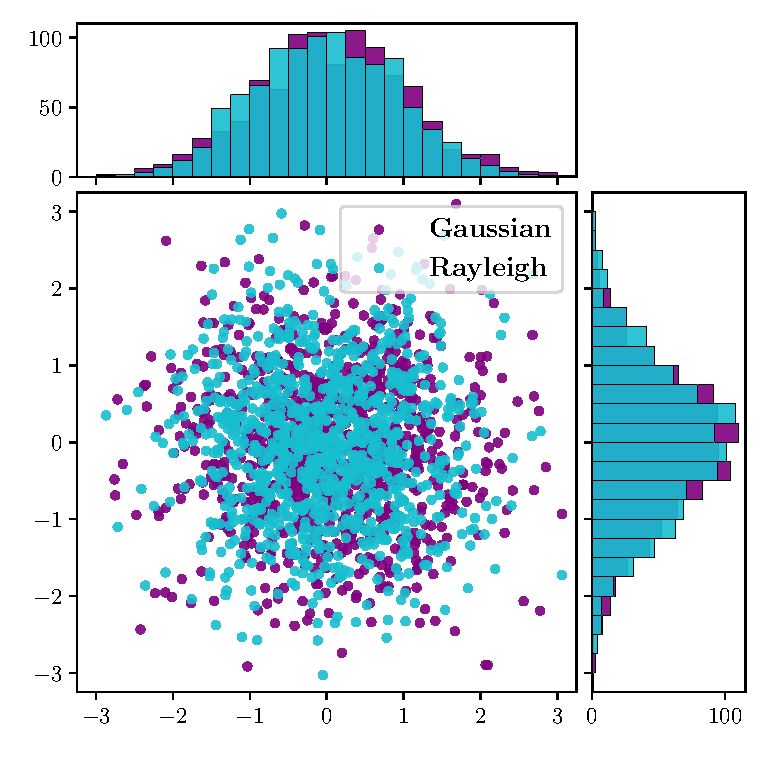
\includegraphics[width=\textwidth]{images/7_rayleigh.pdf}
    \caption{\label{fig:rayleigh} Sampling a 2D Gaussian against a Rayleigh distributed amplitude with uniform complex phase. In purple is the complex number $X+iY$ with $X,Y \sim \mathcal{N}(0,1)$, in cyan is $Re^{i\theta}$ with $R\sim\mathcal{R}(1)$ and $\theta \sim \mathcal{U}(0,2\pi)$.}
\end{figure}

\subsection{Lognormal field}
The universe today is not Gaussian. GRFs are able to capture the 2-point statistics of cosmological fields, but they cannot capture their skewed distribution. A possible way to get closer to the true distribution of the convergence field is with a lognormal transformation \cite{lognormal} \cite{lognormal2} \cite{lognormal3} \cite{fwdmodel}. In this work we will denote lognormal transformations as $\mathcal{L}$ and adopt the following convention for both the field and the correlation function,
\begin{gather}
    \label{eq:L_w}
    \mathcal{L}_w^{-1}(w^{L}, a) \equiv \log \left(\frac{w^{L}}{a^2}+1\right) = w^G,\\
    \label{eq:L_k}
    \mathcal{L}_\kappa(\kappa^G, a) \equiv a\left(\exp(\kappa^G-\tfrac{1}{2}\text{Var}(\kappa^G)) -1\right) = \kappa^{L}.
\end{gather}
Where the superscripts L and G respectively stand for lognormal and Gaussian, Var($\cdot$) stands for the variance of the field and $a$ is the so-called shift parameter, which is an indicator of the non-Gaussianity of the resulting field.

\section{Gaussian process}
\label{sec:gaussian process}
One way to think of Gaussian processes is as an extension of random vectors to infinite dimensions. Following this train of thought, let's begin with the concept of a random variable following a normal distribution. We say,
\begin{equation*}
    X \sim \mathcal{N}\left(\mu, \sigma^2\right),
\end{equation*}
to mean that $X$ is a sample of a Gaussian of mean $\mu$ and variance $\sigma^2$. If we were to get enough samples $X$, we would eventually recover its distribution. The generalisation of this concept to n-dimensions is a collection of random variables, described by a so-called multivariate normal distribution,
\begin{equation*}
    \bm{X} \sim \mathcal{N}\left(\bm{\mu}, \bm{K}\right).
\end{equation*}
Where $\bm{X}=(X_0,X_1,...)$ is a vector of random variables, $\bm{\mu}$ is the mean vector and $\bm{K}$ the covariance matrix. For a zero mean field, the covariance matrix is formed by the variance of each of the random variables on its diagonal, while the cross correlation terms populate the rest of the matrix. 
\subsection{Definition}
Adopting the philosophy of Rasmussen \cite{rasmussen}, functions can be thought of as very long vectors of the form $\left(f(x_1), f(x_2), ...\right)$. Such a view allows us to extend the definition of multivariate Gaussians, to functions. Defining $\mathcal{GP}$ a Gaussian process, a sample function $f$ will be given by:
\begin{equation}
    f(\bm{x}) \sim \mathcal{GP}\left(m(\bm{x}), k(\bm{x}, \bm{x'})\right)
\end{equation}
with $m(\bm{x})$ and $k(\bm{x}, \bm{x'})$ defined as,
\begin{gather}
    m(\bm{x})=\mathbb{E}[f(\bm{x})],\\
    k(\bm{x}, \bm{x'})=\mathbb{E}[(f(\bm{x})-m(\bm{x}))(f(\bm{x}')-m(\bm{x}'))],
\end{gather}
 Mathematically a GP is defined for a continuous function. Computationally this is not possible and we must treat space as a discrete grid. 

\subsection{Prior and posterior samples}
Given some $m(\cdot)$ and $k(\cdot,\cdot)$ which define a GP, a random sample from said GP would be a function $\bm{f}_*$ defined on a domain $D_*$, which is our grid.
\begin{equation}
    \bm{f}_* \sim \mathcal{N}(\bm{m}, \bm{K}_{**}).
    \label{eq:gp prior}
\end{equation}
Here we adopt the convention $\bm{K} = k(D_*,D_*)$. When drawing a sample function from \textit{Eq. }\eqref{eq:gp prior}, computationally the operation is equivalent to drawing a vector from a multivariate Gaussian. What we obtain is a so-called prior, or priors, see \textit{Fig. }\ref{fig:priors}.
\begin{figure}[h]
    \centering
    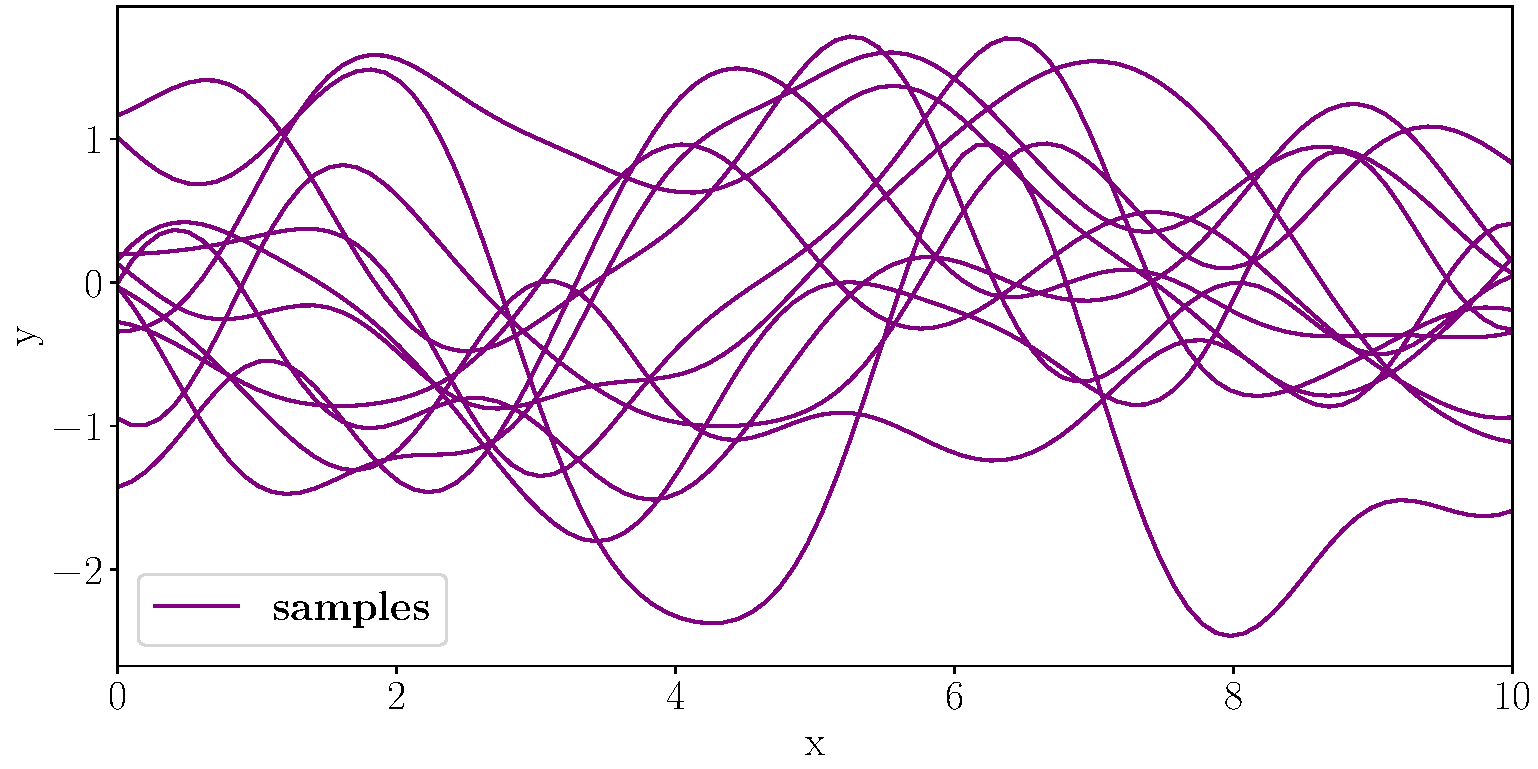
\includegraphics[width=\textwidth]{images/1_priors.pdf}
    \caption{Prior samples of a GP with mean $m(\bm{x})=0$ and squared exponential kernel $k(\bm{x},\bm{x'})=e^{-(\bm{x}-\bm{x'})^2}$.}
    \label{fig:priors}
\end{figure}

Let's now see how we can introduce knowledge of data points in this system. We divide the grid in training points $D$ and test points $D_*$. To each training point is associated a known value $\bm{y}$ and variance $\sigma_n^2$, whereas the values of the function at the test points $\bm{f}_*$ are unknown. We can summarise this as,
\begin{equation}
    \begin{bmatrix}
    \bm{y} \\
    \bm{f}_* \\
    \end{bmatrix}
    \sim \mathcal{N}\left(\bm{m}, \begin{bmatrix}
    \bm{K} + \sigma_n^2 I & \bm{K}_* \\
    \bm{K}^T_* & \bm{K}_{**} \\
    \end{bmatrix}\right)
\end{equation}
where we have once again adopted the notation $\bm{K}=k(D,D)$, $\bm{K_{*}}=k(D,D*)$, $\bm{K_{**}}=k(D_*,D_*)$. At this point, one way to find samples that follow the data would be to blindly draw priors until we get something that goes through all data points. This would be inefficient and computationally wasteful. Instead, we make a better guess for the test function values. This operation is called conditioning, because we condition the joint Gaussians on the training points, this gives
\begin{equation}
\bm{f}_* \mid D_*, D, \bm{y} \sim \mathcal{N}\left( \bm{K}^T_* [\bm{K} + \sigma_n^2 I]^{-1} \bm{y} , \bm{K}_{**} - \bm{K}^T_* [\bm{K} + \sigma_n^2 I]^{-1} \bm{K}_* \right).
\label{eq:conditioning}
\end{equation}
Conditioning can therefore give rise to what is called a posterior sample, \textit{Fig. }\ref{fig:posteriors}. The result is still a multivariate Gaussian, but the mean and variance given by \textit{Eq. }\eqref{eq:conditioning} generate samples that are a better guess of the behaviour of the function outside of the training points.
\begin{figure}[h]
    \centering
    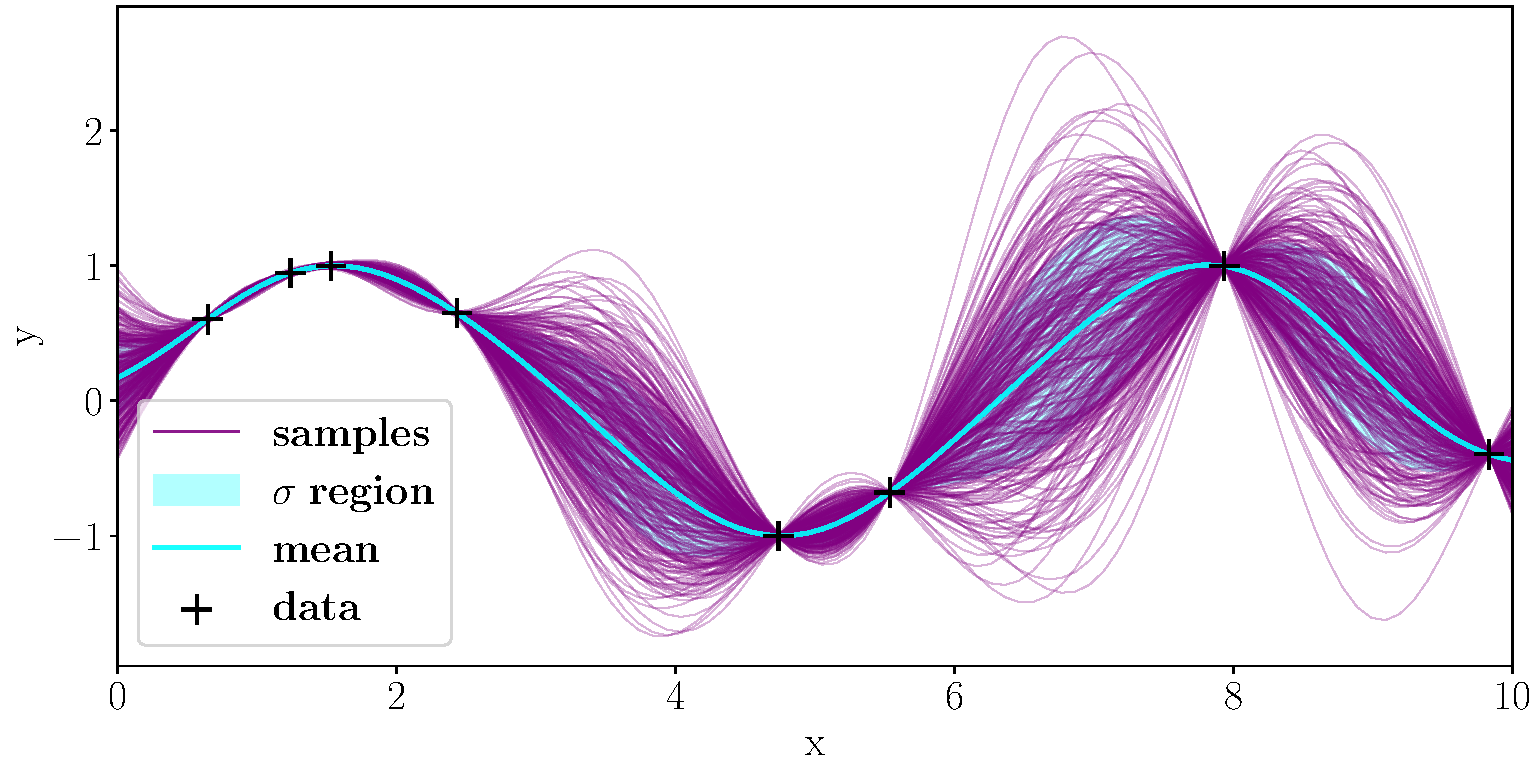
\includegraphics[width=\textwidth]{images/1_posteriors.pdf}
    \caption{\label{fig:posteriors} Summary plot of a GP conditioned to some data. The cyan line is the mean of the GP and the filled region corresponds to $1\sigma$. The purple lines are posterior samples, which are distributed Gaussianly around the mean. The data points are clearly marked in black, they are also the points where all samples converge to.}
\end{figure}

\begin{comment}
\subsection{Likelihood [should I include this?]}
The probability density function of the function values $\bm{f}$ under the Gaussian prior $\bm{f}\mid X \sim \mathcal{N}(\bm{0}, \bm{K})$ is
\begin{equation}
    p(\bm{f\mid X}) \propto \mid\bm{K}\mid^{-{\tfrac{1}{2}}} \exp\left(-{\tfrac{1}{2}} \bm{f}^\mathrm{T} \bm{K}^{-1} \bm{f}\right)
\end{equation}
or
\begin{equation}
    \log p(\bm{f\mid X}) \propto -{\tfrac{1}{2}}\log \mid\bm{K}\mid-{\tfrac{1}{2}} \bm{f}^\mathrm{T} \bm{K}^{-1} \bm{f}
\end{equation}
from here it can be shown that if the data $\bm{y}$ is normally distributed around some value $f$, meaning $\bm{y\mid f}\sim\mathcal{N}(\bm{f}, \sigma_n^2\bm{I})$, then by marginalising over all possible values of $\bm{f}$, we obtain
\begin{equation}
    \log \mathcal{L}(\bm{y\mid X}) \propto -{\tfrac{1}{2}}\log \mid\bm{K}+\sigma_n^2\bm{I}\mid-{\tfrac{1}{2}} \bm{y}^\mathrm{T} (\bm{K}+\sigma_n^2\bm{I})^{-1} \bm{y}.
\end{equation}
\end{comment}